%\documentclass[12pt,preprint]{aastex}
\documentclass[iop,apj]{emulateapj}
%\usepackage{multirow}
\usepackage{longtable}
\usepackage{ulem}
%\usepackage[monochrome]{color}
\usepackage{color}
%\usepackage{lipsum}
\usepackage{amsmath}
%\usepackage{hyperref}

\newcommand{\eqqref}[1]{Equation (\ref{#1})}
\newcommand{\tabref}[1]{Table~\ref{#1}}
\newcommand{\figref}[1]{Figure~\ref{#1}}
\newcommand{\secref}[1]{Section~\ref{#1}}
\newcommand{\appref}[1]{Appendix~\ref{#1}}

\newcommand{\SNeIa}{SNe~Ia}
\newcommand{\SNIa}{SN~Ia}
\newcommand{\C}[1]{\ensuremath{{}^{#1}{\rm C}}}
\newcommand{\Ox}[1]{\ensuremath{{}^{#1}{\rm O}}}
\newcommand{\Ne}[1]{\ensuremath{{}^{#1}{\rm Ne}}}
\newcommand{\Na}[1]{\ensuremath{{}^{#1}{\rm Na}}}
\newcommand{\Mg}[1]{\ensuremath{{}^{#1}{\rm Mg}}}
\newcommand{\Ni}[1]{\ensuremath{{}^{#1}{\rm Ni}}}
\newcommand{\Co}[1]{\ensuremath{{}^{#1}{\rm Co}}}
\newcommand{\Si}[1]{\ensuremath{{}^{#1}{\rm Si}}}
\newcommand{\Fe}[1]{\ensuremath{{}^{#1}{\rm Fe}}}
\newcommand{\code}[1]{\textsc{#1}}
\newcommand{\FLASH}{\code{FLASH}}
\newcommand{\CASTRO}{\code{CASTRO}}
\newcommand{\MESA}{\code{MESA}}
\newcommand{\PARAMESH}{\code{PARAMESH}}
\newcommand{\pv}{\ensuremath{\phi}}
\newcommand{\bvec}[1]{\ensuremath{\boldsymbol{#1}}} %boldface vector style
\newcommand{\grad}{\bvec{\nabla}} %gradient
\newcommand{\curl}{\bvec{\nabla \times}} %curl
\newcommand{\Atwood}{\ensuremath{\mathrm{At}}}
\newcommand{\adndt}{At.~Data~Nucl.~Data~Tables}
\newcommand{\At}{{\rm At}}
\newcommand{\ee}[1]{\ensuremath{\times 10^{#1}}}
\newcommand{\cdens}{\rho_{c}}

% basic unit typesetteing
\newcommand{\unitspace}{\ensuremath{\,}}
\newcommand{\usp}{\unitspace}
\newcommand{\numberspace}{\ensuremath{\;}}
\newcommand{\nsp}{\numberspace}
\newcommand{\unitstyle}[1]{\ensuremath{\mathrm{#1}}}
\newcommand{\power}[2]{\ensuremath{{#1}^{#2}}}


% prefixes
\newcommand{\nano}{\unitstyle{n}}
\newcommand{\milli}{\unitstyle{m}}
\newcommand{\centi}{\unitstyle{c}}
\newcommand{\kilo}{\unitstyle{k}}
\newcommand{\Mega}{\unitstyle{M}}
\newcommand{\Giga}{\unitstyle{G}}

% base units, mks
\newcommand{\meter}{\unitstyle{m}}
\newcommand{\kilogram}{\kilo\gram}
\newcommand{\second}{\unitstyle{s}}

\newcommand{\Kelvin}{\unitstyle{K}}
\newcommand{\K}{\Kelvin}  %degrees Kelvin


% base units, cgs
\newcommand{\cm}{\centi\meter}
\newcommand{\gram}{\unitstyle{g}}


% derived units
\newcommand{\grampercc}{\gram\usp\power{\cm}{-3}} %mass density
\newcommand{\grampersquarecm}{\gram\usp\power{\cm}{-2}} %column depth
\newcommand{\GramPerCc}{\grampercc}
\newcommand{\GramPerSc}{\grampersquarecm}
\newcommand{\columnunit}{\grampersquarecm}
\newcommand{\dyne}{\unitstyle{dyn}} %dyne
\newcommand{\erg}{\unitstyle{ergs}} %ergs
\newcommand{\ergs}{\erg}
\newcommand{\gauss}{\unitstyle{G}} %gauss
\newcommand{\ergspersecond}{\erg\unitspace\power{\second}{-1}}
\newcommand{\ergspergram}{\erg\unitspace\power{\gram}{-1}}
\newcommand{\cgsflux}{\erg\unitspace\power{\cm}{-2}\usp\power{\second}{-1}}
\newcommand{\kms}{\kilo\meter\unitspace\power{\second}{-1}}

% Nuclear and atomic units
\newcommand{\amu}{\unitstyle{u}} %atomic mass unit
\newcommand{\angstrom}{\mbox{\AA}} %Angstrom
\newcommand{\fermi}{\unitstyle{fm}} %fermi
\newcommand{\eV}{\unitstyle{eV}}        %eV
\newcommand{\keV}{\kilo\eV} %Kev
\newcommand{\MeV}{\Mega\eV} %MeV

% solar and astronomical units
\newcommand{\Msun}{\ensuremath{M_\odot}}
\newcommand{\Myr}{\Mega\yr}
\newcommand{\Gyr}{\Giga\yr}
\newcommand{\parsec}{\unitstyle{pc}}
\newcommand{\kpc}{\kilo\parsec} %kiloparsec
\newcommand{\mJy}{\unitstyle{\mu Jy}} %micro Jansky

% misc. units
\newcommand{\minute}{\unitstyle{min}} %minute
\newcommand{\hour}{\unitstyle{hr}} %hour
\newcommand{\yr}{\unitstyle{yr}}        %year
\newcommand{\km}{\kilo\meter}   %kilometers
\newcommand{\Hz}{\unitstyle{Hz}}        %Hertz
\newcommand{\ksec}{\kilo\second} %kilosecond

\newcommand{\tDDT}{\ensuremath{t_{\rm DDT}}}
\newcommand{\rhoDDT}{\ensuremath{\rho_{\rm DDT}}}
\newcommand{\COreac}{\ensuremath{\C{12}\left(\alpha,\gamma\right)\Ox{16}}}

\bibliographystyle{apj}

\shorttitle{Hybrid Ia Progenitors}

\begin{document}

\title{Type Ia Supernova Explosions from Hybrid Carbon-Oxygen-Neon White Dwarf Progenitors}

\author{
Carlyn N.\ Augustine\altaffilmark{1},
Donald E.\ Willcox\altaffilmark{2},
Dean M.\ Townsley\altaffilmark{3},
and Alan C.\ Calder\altaffilmark{2,4}
}

\altaffiltext{1}{
  Department of Physics and Astronomy,
  The University of Alabama, Tuscaloosa, AL, 35487-0324, USA
}
\altaffiltext{2}{
  Department of Physics and Astronomy,
  Stony Brook University, Stony Brook, NY, 11794-3800, USA; \\
  \href{mailto:donald.willcox@stonybrook.edu}{donald.willcox@stonybrook.edu}
}
\altaffiltext{3}{
  Institute for Advanced Computational Sciences,
  Stony Brook University, Stony Brook, NY, 11794-5250, USA
}

\begin{abstract}
Recent studies of stellar evolution predict the existence of "hybrid" white 
dwarfs, made of a C/O/Ne
core within a O/Ne shell, and that these are viable progenitors for supernovae.
More recent work found that the C/O core is mixed with the surrounding O/Ne
while the white dwarf cools. Inspired by this scenario, we performed simulations of
thermonuclear supernovae from these hybrid progenitors. The progenitor model 
was constructed with the one-dimensional stellar evolution code MESA and
represented a star evolved through the phase of unstable interior mixing 
followed by accretion until it reached conditions for the ignition of 
carbon burning. The MESA model was then mapped to a two-dimensional initial 
condition and an explosion simulated with FLASH. For comparison, a similar
simulation of an explosion was performed from a traditional C/O progenitor
white dwarf. By comparing the yields of the explosions, we found....
how explosions from these models differ from explosions from previous models
without the mixing during the white dwarf cooling.
\end{abstract}

\keywords{hydrodynamics --- nuclear reactions, nucleosynthesis, abundances
--- supernovae: general --- white dwarfs}

%%%%%%%%%%%%%%%%%%%%%%%%%%%%%%%%%%%%%%%%%%%%%%%%%%%%%%%%%%%%%%%%%%
\section{Introduction}
\label{sec:intro}
Thermonuclear (Type Ia) supernovae (\SNeIa) are bright stellar explosions 
thought to occur when approximately 1.X \Msun of material composed principally 
of C and O burns under degenerate conditions (SETTLE ON X). This class of supernovae is
know to synthesize much of the Fe-group elements found in the galaxy and
the light curves of these events have a spectial property that allows
their use as distance indicators for cosmological studies~\citep{phillips:absolute}
resulting in the discovery of the acceleration of the expansion of
the Universe and thus the inference of Dark 
Energy~\citep{riess.filippenko.ea:observational,
perlmutter.aldering.ea:measurements,leibundgut2001}. 
This special property of the light curve is thought to follow
from the fact that the source of luminosity, the radioactive decay
of \Ni{56}, synthesized by the thermonuclear burning, is also the
principle source of opacity~\citep{Pinto2001The-type-Ia-sup}. 

Supernovae are classified observationally 
by their light curves and spectra~\citep{minkowski41,bertola64,porterfilippenko87,
wheelerharkness1990conf,Fili97}, with the type Ia designation following from
the absence of H in the spectrum and the presence of a specific Si 
line~\citep{filippenko:optical,hillebrandt.niemeyer:type}. These events
have been associated with C burning under degenerate conditions
for some time~\citep{hoylefowler60,arnett.truran.ea:nucleosynthesis},
but discerning the setting(s) of these events is proving difficult
and remains the subject of active research. At present there are three
widely-accpeted scenarios: the {\em single degenerate} scenario,
the {\em double detonation} or {\em sub-Chandrasekhar} scenario, 
the {\em white dwarf merger} or {\em double degenerate} scenario.
We briefly describe these in the subsection that follows. `
Also see~\citet{hillebrandt.niemeyer:type,howell2011,hillebrandtetal2013,calderetal2013}
for additional discussion.

\subsection{Proposed Progenitor Settings}

The single degenerate picture posits a white dwarf gaining mass
from a main-sequence companion. The process relies on a long
period of accretion combined with either steady burning or a 
series of nova explosions to allow the WD to gain
~0.6 CHECK THIS \Msun needed for it to approach the
limiting Chandrasekhar mass~\citep{starrfieldetal2012}. As it approaches
the Chandrasekhar limit, conditions in the compressed core are right
to ignite the thermonuclear buring that will incinerate the star. Within this
progenitor setting, the models that best reproduce the observed
stratified ejecta are those in which the burning begins as a 
subsonic deflagration, which allows the star to react and expand
thus lowering the density, that is followed by a 
detonation~\citep{Nomo84,Khokhlov1991Delayed-detonat,HoefKhok96,GameKhokOran05}.
We adopt this setting for the explosion simulations we present and 
describe our approach in detail below. 

The double detionation picture is a variation of the single degenerate picture.
In this case, a white dwarf accretes material from a companion, but rather
than gaining enough mass to approach the Chandrasekhar limit, a detonation
occurs in the accreted layer that subsequently triggers a detonation
in the underlying white dwarf \citet{woosleyweavertaam80,taam80a,taam80b,
nomoto80,nomoto82b}. Early studies indicated that a detonation in an 
accreted He
layer could produce an inwardly propagating
shock that would ignite a detonation in the C-O core and found
that this scenario could work for a wide range of white dwarf
masses, not just the near-Chandrasekhar case \citep{livne90}, hence the
moniker ``sub-Chandrasekhar'' \citep{ww94}. Multidimensional supported the
efficacy of this picture~\citep{livneglasner91, livnearnett95,HoefKhok96,
hoeflichetal96, wigginsfalle97,wigginsetal98,garciasenzbravowoosley99} 
but indicated that uncertainties 
like the initial conditions were found to play a significant role.
on the explosion outcome. 

A particular problem was that most models 
included a massive He layer, which leads to 
the unobserved result intermediate and heavy elements synthesized in 
the He detonation in the outer parts of the ejecta~\citep{HoefKhok96, 
hoeflichetal96,finkhillebrandtroepke2007,simetal2010}.
\citet{bildstenetal2007}, however, found that fairly thin He layers
could flash on sub-Chandrasekhar
mass white dwarfs, partially resolving the issue and encouraging
further research~\citep{simetal2012,brooksetal2015, shenetal2018,
glasneretal2018}.

The white dwarf merger progentor picture has two white dwarfs coming 
together and subsequently exploding~\citep{tutukovyungelson76,tutukovyungelson79,
webbink84,ibentutukov84}. This scenario provides an abundance of degenerate fuel, 
which may explain some bright events~\citep{scalzo:2010,Yuan:2010}. 
An early concern about this model came from studies finding that
the white dwarf will ignite at the edge and the coalesced object, 
and a flame will burn inward, converting the C-O white dwarf into 
an O-Ne-Mg white dwarf~\citep{saionomoto1985,saionomoto2004}, with
further accretion leading to the collapse of the white dwarf
into a neutron star, a scenario termed ``accretion-induced collapse''
\citep{nomotokondo1991}.

Subsequent work allayed this concern~\citep{yoonetal2007,lorenaguilaretal2009,
Shenetal12, pakmoretal2012b} and motivated by the need to expain briht events
and the estimated population WD pairs, active research continues. Contemporary
research focuses on variations on the merger idea, including 
inspiraling pairs, collisions, violent mergers,
and the ``core-degenerate'' model in which the merger takes place in
a common envelope \citep{raskinetal2009,pakmoretal2011,kashi:2011,pakmoretal2012a,Shenetal12,katzetal2016}.






\subsection{The near-Chandrasekhar-mass Single Degenerate Scenario}



In our study, we use the single degenerate process to ignite a flame. The
flame in the core starts out in the deflagration process, sub sonically
burning C/O/Ne in its path. Once it reaches a certain density, the
wave moves into the detonation front and sweeps through the rest of
the star. This process is the deflagration to detonation process (DDT):
when a wave moves from being subsonic to supersonic.

Carlyn's starter text: (to end starter)

The fuel starts off cold. The elections in the plasma conduct heat
and the fuel begins to heat up. Once the fuel reaches a certain
temperature, the reaction starts. The fuel abundance begins to
decline because it is consuming fuel. Energy is produced which
makes the fuel hot. Eventually, all that’s left is ash. As
surface area grows, conducted energy increases and density
decreases. At low densities Rayleigh-Taylor instability causes
the flame to get more tangled and unstable. Eventually, the
star will get a large enough surface area in this volume that
the net burning effect is supersonic. Therefore, the transition
from deflagration to detonation is made.

A deflagration alone will not produce an event of normal
brightness and expansion velocity. Instead, the initial
deflagration must transition to a detonation after the star has
expanded some in order to produce abundances and a stratified
ejecta in keeping with observations. The physics of this
“deflagration-to- detonation transition” (DDT) are not
completely understood, but there has been considerable study
based on mechanisms involving flame fronts in highly turbulent
conditions. These models generally reproduce the observations
under certain assumptions about the ignition, but research has
shown that the results are very sensitive to the details of the
ignition. In our simulations, we initialize a detonation once
the deflagration front reaches a characteristic DDT fuel density,
which controls the degree of expansion the star undergoes during
the deflagration stage.

The comparison study of tradition C/O progenitor WDs used the same initial
conditions for the realizations within the suite. The traditional models
are simulated with the same code and the same set of perturbations on the
initial match head (realization). The only difference is the different
nuclear burning to include the other Ne and the initial profile of the
1-d model. 

(end starter)


Explain the Single Degenerate scenario
\citep{Baraffe2004Stability-of-Su,WoosWunsKuhl04,wunschwoosley2004,Kuhletal06,nonakaetal2012}.
expansion \citep{Nomo84,WoosWunsKuhl04}, and a flame is born. 

Explain DDT

Go through below and cite some of these as you tell the story

d~\citep{arnett.truran.ea:nucleosynthesis}.
~\citep{mazzalietal2008}.  


\citep{khokhlov1993,bychovliberman1995,
SNrt,Khok95,NiemHill95,khoketal1997,ZingDurs07,
cholazarianvishniac2003,
roepkehn2003,roepkehn2004,
Zingale2005Three-dimension,Schmetal06a, Schmetal06b,Aspdetal08,
Woosetal09,csetal2009,hicksrosner2013,c-ssr2013,
jacketal2014,poludnenko2015,hicks2015}.


A deflagration alone will not produce a event of normal brightness and
expansion velocity~\citep{roepkeetal07}. Instead, the initial
deflagration must transition to a detonation after the star has
expanded some in order to produce abundances and a stratified ejecta
in keeping with
observations~\citep{Khokhlov1991Delayed-detonat,hokowh95}.
The physics of this ``deflagration-to-detonation transition'' (DDT)
are not completely understood, but there has been considerable study
based on mechanisms involving flame fronts in highly turbulent
conditions~\citep{1986SvAL, woosley90, Khokhlov1991Delayed-detonat,
  hokowh95, HoefKhok96, khoketal1997, NiemWoos97, hwt98, Niem99,
  GameKhokOran05,roepke07, poletal2011,c-ssr2013,poludnenko2015}.
These models generally reproduce the observations under certain
assumptions about the ignition~\citep{townetal2009}, but research has
shown that the results are very sensitive to the details of the
ignition~\citep{PlewCaldLamb04,GameKhokOran05,garciasenz:2005,
  roepkeetal07,Jordan2008Three-Dimension}.

\subsection{A Recent Advance in Stellar Evolution: Hybrid White Dwarfs}

Hybrid models 
old 
\citep{denissenkovetal2015}
\citet{Wangetal2014} and \citet{Mengetal2014} presented binary

Recent results from stellar evolution
The models we are exploding \citep{brooksetal2017}

If we refer to the work by name, it should appear ``The hybrid models
of~\citet{brooksetal2017}." Or, we can just cite it~\citep{brooksetal2017}.

Here's the other Books paper \citep{brooksetal2016}. Do we need to mention it?
Give a read to see!


\section{Methods}

Summarize what we do a la:
In our simulations, we initialize a detonation once the 
deflagration front reaches a
characteristic DDT fuel density, which controls the degree of
expansion the star undergoes during the deflagration stage.

The comparison study of tradition C/O progentor WDs used the same
initial conditions for the realizations within the suite. Make the
point that the traditional models are simalted with the same code
and the same set if perturbations on the initial match head (that is
what we mean by a realization). The only difference is the different
nuclear buring to include the other Ne and the initial profile of
the 1-d model.  

For much of the methodology to be described below, just say a few
words about what was done and cite \citet{willcoxetal2016}.

\subsection{Initial Conditions}

We used MESA, a 1-D stellar evolution code, to create the hybrid
model. We made the hybrid model have the same central temperature
and density as the classic model.

We found that the most abundant isotopes in the model were C12, O16,
Ne20. There were a few other isotopes that were added to form Ne22
later. We saw that  ….

Plotting the density verses solar radii, we found that the densest part
of the star is in the center slowly decreasing until it hits 0 at the
outer edge of the star.

In order to see where we should ignite the flame, we plotted the
temperature profile. It was found that the peak temperature is at the
center of the star, therefore, it was obvious to ignite the flame in
the core. (PUT IN TEMP PROFILE)

\subsection{Created 2D model from 1-D model}

We mapped our hybrid model to the FLASH grid. In order to convert our 1-D
MESA model into FLASH, which is a 2-D code, we needed symmetric nuclear
matter. This means that the ratio of neutrons to protons in the nuclei
must be the same ratio as in the mesa profile. This is because the amount
of extra neutrons around is important when burning the star because that
determines how much neutron rich isotopes the burning produces.


\subsection{DDT Process and Suits of Explosions}

The fuel starts off cold. The elections in the plasma conduct heat and the
fuel begins to heat up. Once the fuel reaches a certain temperature, the
reaction starts. The fuel abundance begins to decline because it is consuming
fuel. Energy is produced which makes the fuel hot. Eventually, all that’s
left is ash. As surface area grows, conducted energy increases and density
decreases. At low densities Rayleigh-Taylor instability causes the flame to
get more tangled and unstable. Eventually, the star will get a large enough
surface area in this volume that the net burning effect is supersonic.
Therefore, the transition from deflagration to detonation is made. 

Using the FLASH code from University of Chicago, simulations of
explosions were preformed. For each simulation we varied the central
ignition seed. 

----updated text-----

DDT Process:
The fuel starts off cold. The elections in the plasma conduct heat
and the fuel begins to heat up. Once the fuel reaches a certain
temperature, the reaction starts. The fuel abundance begins to
decline because it is consuming fuel. Energy is produced which
makes the fuel hot. Eventually, all that’s left is ash. As
surface area grows, conducted energy increases and density
decreases. At low densities Rayleigh-Taylor instability causes
the flame to get more tangled and unstable. Eventually, the
star will get a large enough surface area in this volume that
the net burning effect is supersonic. Therefore, the transition
from deflagration to detonation is made.

A deflagration alone will not produce an event of normal
brightness and expansion velocity. Instead, the initial
deflagration must transition to a detonation after the star has
expanded some in order to produce abundances and a stratified
ejecta in keeping with observations. The physics of this
“deflagration-to- detonation transition” (DDT) are not
completely understood, but there has been considerable study
based on mechanisms involving flame fronts in highly turbulent
conditions. These models generally reproduce the observations
under certain assumptions about the ignition, but research has
shown that the results are very sensitive to the details of the
ignition. In our simulations, we initialize a detonation once
the deflagration front reaches a characteristic DDT fuel density,
which controls the degree of expansion the star undergoes during
the deflagration stage.

The comparison study of tradition C/O progenitor WDs used the same initial
conditions for the realizations within the suite. The traditional models
are simulated with the same code and the same set of perturbations on the
initial match head (realization). The only difference is the different
nuclear burning to include the other Ne and the initial profile of the
1-d model.

----above updated text-----



\section{Results}

A plot of the estimated Ni56 yield as a function of the final, burned mass
for all CO and Hybrid runs. The Hybrid model is shown in red, and the CO
model is shown in blue. As it is shown, the CO model has a higher final mass
then the Hybrid model. 

\begin{figure}
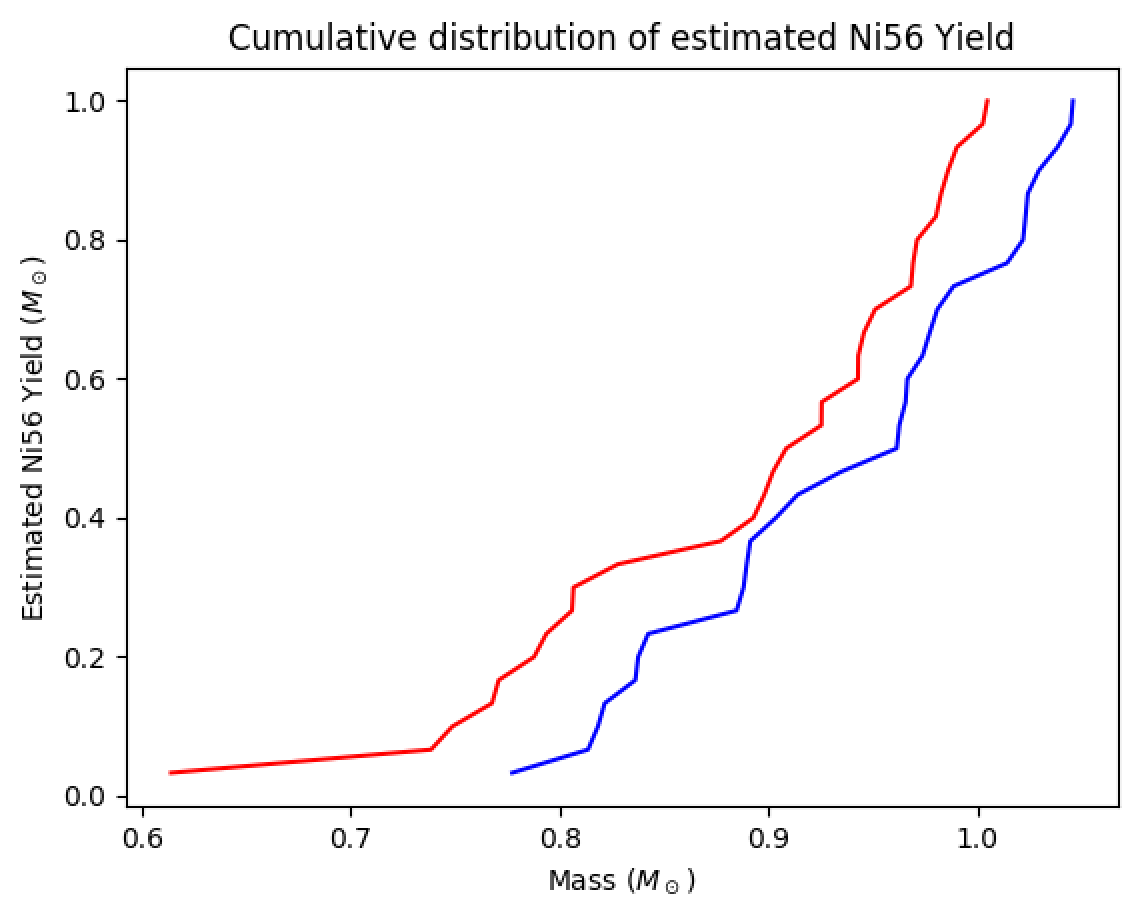
\includegraphics[width=\columnwidth]{figures/ni56_yield_cum_dist.png}
\caption{\label{fig:cumdist}
A plot of the estimated Ni56 yield as a function of the final, burned mass
for all CO and Hybrid runs. The Hybrid model is shown in red, and the CO
model is shown in blue. As it is shown, the CO model has a higher final mass
then the Hybrid model. 
}
\end{figure}

\begin{figure}
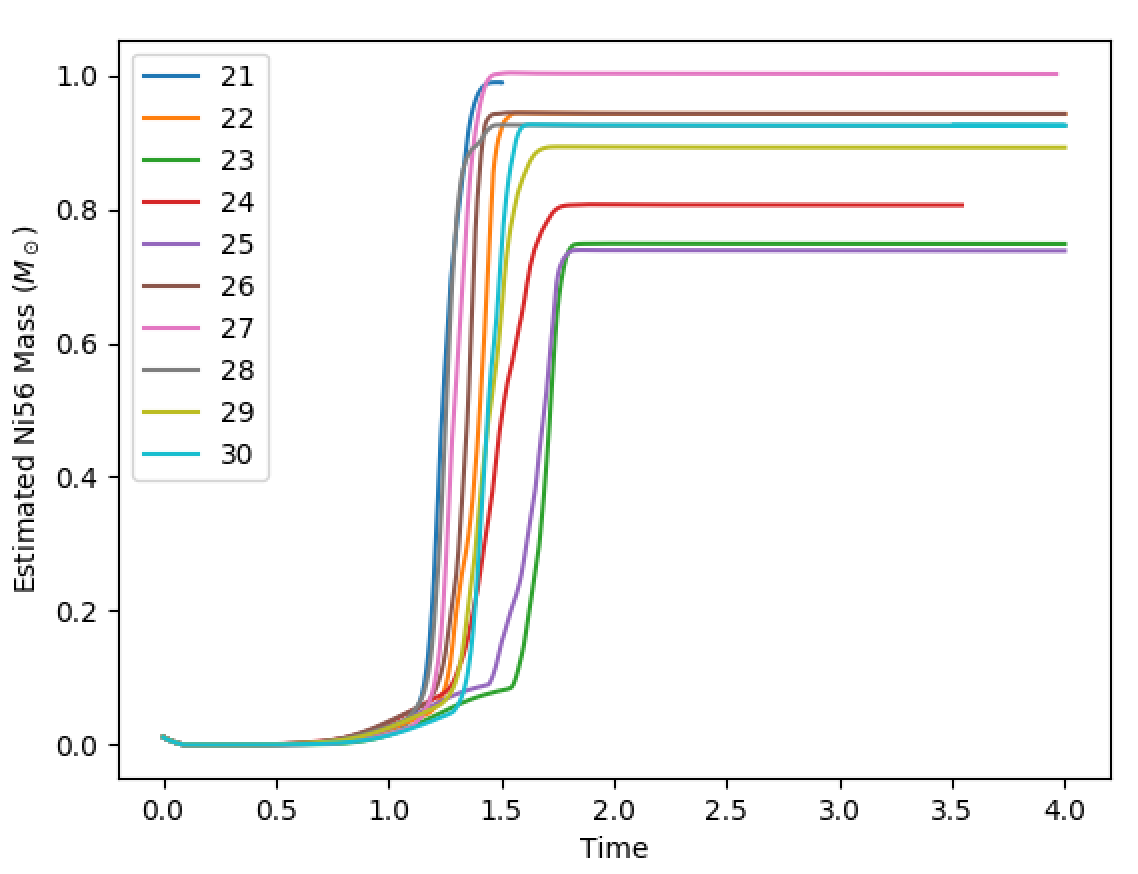
\includegraphics[width=\columnwidth]{figures/ni56_vs_time_hybrid.png}
\caption{\label{fig:nithybrid}
Estimated Ni56 mass for Hybrid Model
}
\end{figure}

\begin{figure}
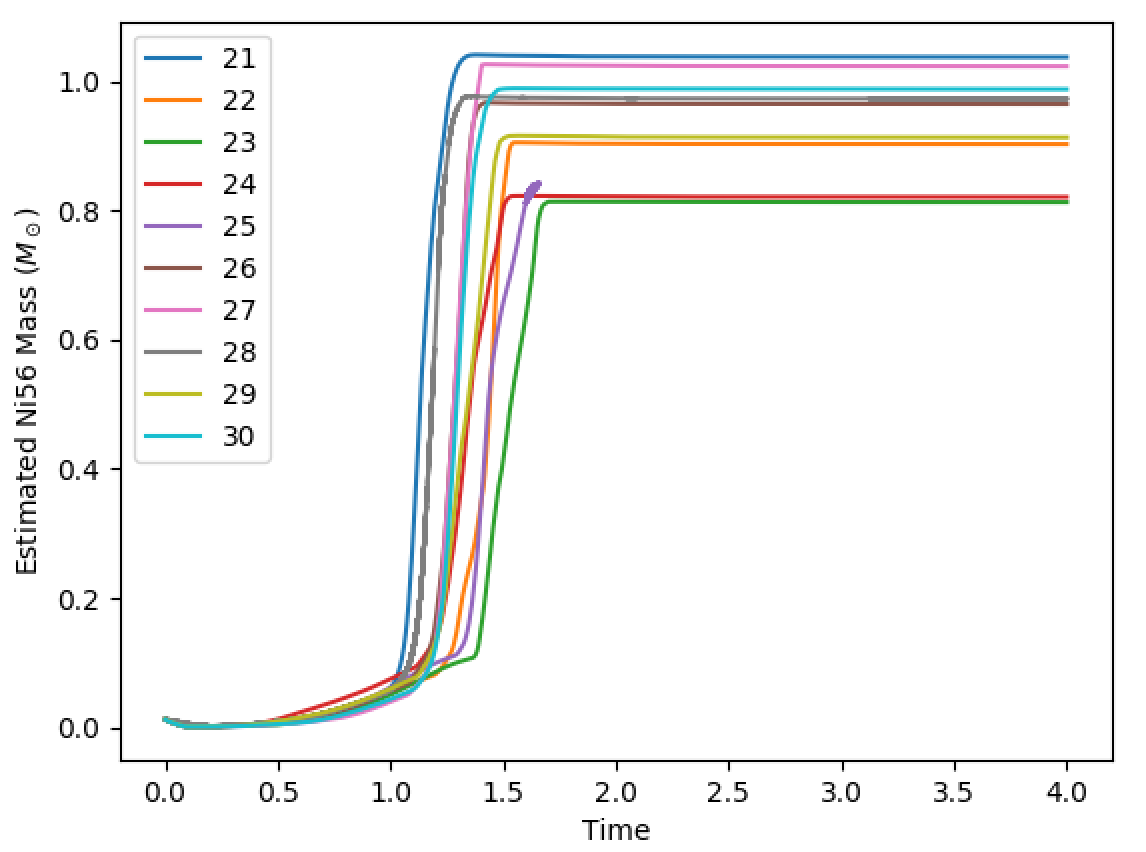
\includegraphics[width=\columnwidth]{figures/ni56_vs_time_CO.png}
\caption{\label{fig:nitco}
Estimated Ni56 mass for CO Model
}
\end{figure}

The figures show that the final Estimated Ni56 for the CO model is
slightly larger then the Hybrid model. Therefore, the CO produces more
Ni56. The Hybrid model has a larger range then the CO model. Also, on
average, the CO model reaches the DDT phase sooner then the Hybrid model.


This is a plot of the estimated Ni56 yield vs. mass below 2e7 g/cc at
the time of the DDT.

The degree of expansion was found using the time at which the first
detonation point occurred, and the mass at density less then 2e7 g/cc. The
estimated Ni56 Yield is the final estimated mass of the model.

\begin{figure}
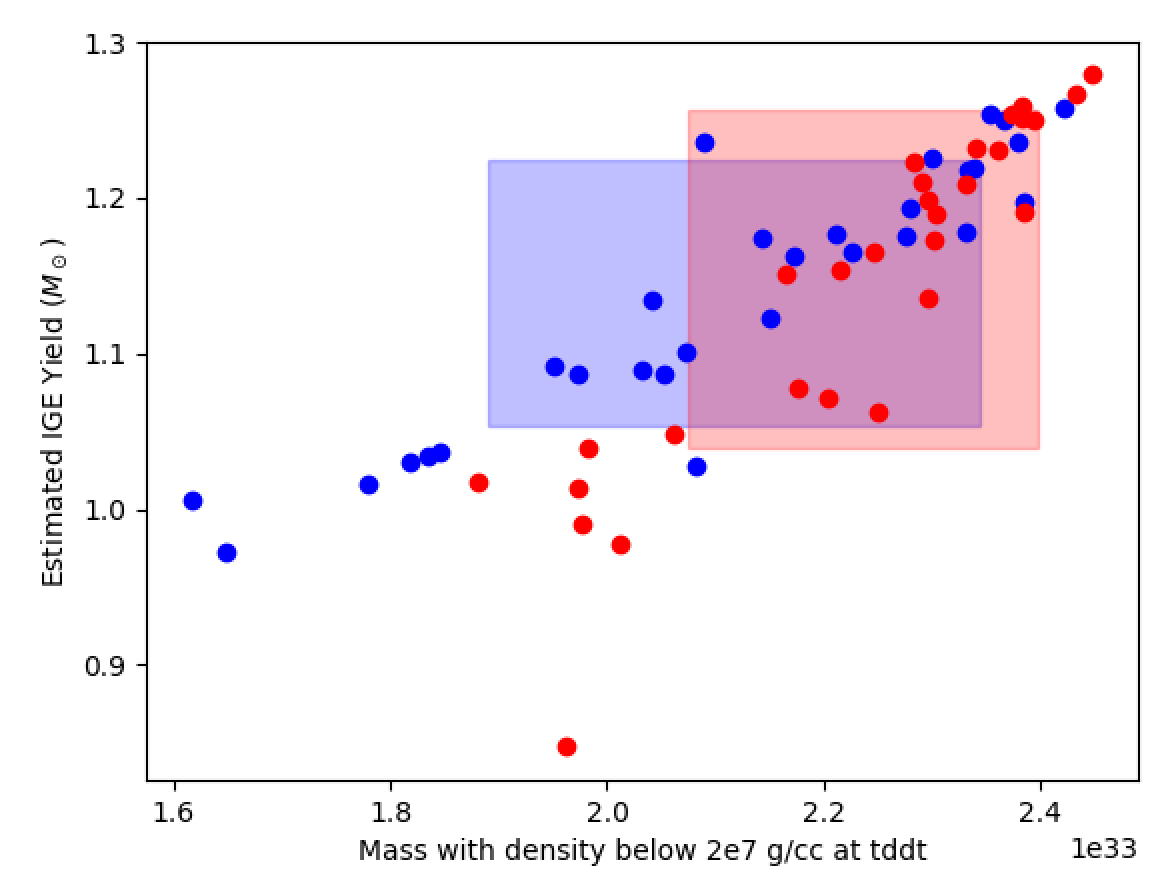
\includegraphics[width=\columnwidth]{figures/ni56_yield_vs_mass_at_high_dens_v2.png}
\caption{\label{fig:masshighdens}
...
}
\end{figure}

\section{Discussion and Conclusion}


The conversion of Ni56 to Iron group elements are more pronounced in my
case. There are two assumptions as to why figure 6 is more pronounced
in my paper then in Dons.  First is that higher critical density leads
to higher electron capture resulting in less Ni56 produced. The second
is that the central ignition leads to early burning at higher density.


As the star burns mass, the surface area grows, resulting in a decrease
in density. The results show that the models that burned less mass during
the deflagration phase, expand less, produce more Ni-56. This is because
the density rich mass the model has at the DDT point is the ‘fuel’
it needs to produce Ni-56. Therefore, the more mass, the more Ni-56. On
average, the CO model, shown in figure 4, reaches the DDT faster then
the hybrid model. Figures 3 and 4 show that the hybrid model has a wider
range of estimated Ni-56 mass suggesting a greater range of burned mass
and expansion during the deflagration phase.




This work was supported in part by the Department of Energy under
grant DE-FG02-87ER40317. The software used in this work was in part
developed by the DOE-supported ASC/Alliances Center for Astrophysical
Thermonuclear Flashes at the University of Chicago. Results in this
paper were obtained using the high-performance computing system at the
Institute for Advanced Computational Science at Stony Brook
University.  other grants...

%%%%%%%%%%%%%%%%%%%%%%%%%%%%%%%%%%%%%%%%%%%%%%%%%%%%%%%%%%%%%%%%%%
% SOFTWARE
%% \software{
%%   FLASH \citep{Fryxetal00},
%%   CASTRO \citep{castro1},
%%   MESA \citep{mesa1},
%%   Matplotlib \citep{http://dx.doi.org/10.5281/zenodo.44579}
%% }

%%%%%%%%%%%%%%%%%%%%%%%%%%%%%%%%%%%%%%%%%%%%%%%%%%%%%%%%%%%%%%%%%%
\bibliography{master}


\end{document}

